\documentclass[aspectratio=169]{beamer}

% Shared Beamer settings for Applied Machine Learning lectures (UPES).
% Keep this file free of \documentclass to allow reuse via \input.

% Allow lecture sources to use shared theme/assets without copying them into each lecture folder.
% NOTE: These paths are relative to `Unit-xx/Lecture-yy/latex/` (and `Lab/Experiment-xx/latex/`).
\makeatletter
\def\input@path{{../../../_shared/}{../../../_shared/UPES-Beamer-Theme/}}
\makeatother

\usetheme{UPES}
\setbeamertemplate{navigation symbols}{}

\usepackage{amsmath}
\usepackage{amssymb}
\usepackage{booktabs}
\usepackage{graphicx}
\usepackage{hyperref}
\usepackage{xcolor}
\usepackage{listings}

% Code listings (Python-oriented for this subject).
\lstset{
  language=Python,
  basicstyle=\ttfamily\small,
  keywordstyle=\color{blue},
  commentstyle=\color{gray},
  stringstyle=\color{teal},
  showstringspaces=false,
  columns=fullflexible,
  breaklines=true
}

\usepackage{tikz}
\usetikzlibrary{arrows.meta,positioning,shapes.geometric,calc,fit,backgrounds}

% Per-slide source line (references shown on the slide itself).
\newcommand{\slidesources}[1]{%
  \vfill
  {\tiny\color{gray}\raggedright\sloppy\parbox{\linewidth}{Sources: #1}\par}%
}

% Unit-wise source strings for this subject (used by slides/notes).
% Path is relative to the lecture `latex/` folder (the compilation CWD).
% Source strings for Applied Machine Learning (CSAI2017P) — used by slides + notes.
% Prescribed texts and reference books are taken from the course syllabus.
% Support texts are the author-hosted open-access editions:
%   statlearning.com            (ISL with Python)
%   probml.github.io/pml-book   (Murphy, Probabilistic Machine Learning)
%   d2l.ai                      (Dive into Deep Learning)
%   mml-book.github.io          (Mathematics for Machine Learning)

\newcommand{\AMLRepoURL}{https://github.com/tali7c/Applied-Machine-Learning}

% --- prescribed -------------------------------------------------------------
\newcommand{\AMLPrescribed}{%
M\"uller and Guido, \textit{Introduction to Machine Learning with Python}, O'Reilly, 2016.;%
Bishop, \textit{Pattern Recognition and Machine Learning}, Springer, 2006.;%
Murphy, \textit{Machine Learning: A Probabilistic Perspective}, MIT Press, 2012.;%
Han, Kamber and Pei, \textit{Data Mining: Concepts and Techniques} (3e), Morgan Kaufmann, 2012.%
}

% --- unit-wise ---------------------------------------------------------------
\newcommand{\AMLUnitISources}{%
M\"uller and Guido, \textit{Introduction to Machine Learning with Python}, Ch. 1.;%
Bishop, \textit{Pattern Recognition and Machine Learning}, Ch. 1.;%
Murphy, \textit{Probabilistic Machine Learning: An Introduction}, MIT Press, 2022, Ch. 1.;%
Mitchell, \textit{Machine Learning}, McGraw Hill, 1997, Ch. 1.;%
Scikit-learn documentation, accessed 2026-08-04.%
}

\newcommand{\AMLUnitIISources}{%
Bishop, \textit{Pattern Recognition and Machine Learning}, \S1.5, \S4.3, \S7.1.;%
Zhang, Lipton, Li and Smola, \textit{Dive into Deep Learning}, \S3.4.;%
Shalev-Shwartz and Ben-David, \textit{Understanding Machine Learning}, Ch. 15.;%
Murphy, \textit{Probabilistic Machine Learning: An Introduction}, Ch. 5.%
}

\newcommand{\AMLUnitIIISources}{%
Zhang, Lipton, Li and Smola, \textit{Dive into Deep Learning}, Ch. 12 (Optimization Algorithms).;%
Deisenroth, Faisal and Ong, \textit{Mathematics for Machine Learning}, Ch. 7.;%
Kingma and Ba, ``Adam: A Method for Stochastic Optimization,'' ICLR 2015.;%
Ruder, ``An overview of gradient descent optimization algorithms,'' arXiv:1609.04747, 2016.%
}

\newcommand{\AMLUnitIVSources}{%
Han, Kamber and Pei, \textit{Data Mining: Concepts and Techniques} (3e), Ch. 3.;%
M\"uller and Guido, \textit{Introduction to Machine Learning with Python}, Ch. 3--4.;%
James, Witten, Hastie, Tibshirani and Taylor, \textit{An Introduction to Statistical Learning with Python}, Ch. 5--6, 12.;%
Scikit-learn documentation (preprocessing, model selection), accessed 2026-08-04.%
}

\newcommand{\AMLUnitVSources}{%
James et al., \textit{An Introduction to Statistical Learning with Python}, Ch. 3--6.;%
Bishop, \textit{Pattern Recognition and Machine Learning}, Ch. 3.;%
Deisenroth, Faisal and Ong, \textit{Mathematics for Machine Learning}, Ch. 9.;%
M\"uller and Guido, \textit{Introduction to Machine Learning with Python}, \S2.3.%
}

\newcommand{\AMLUnitVISources}{%
Han, Kamber and Pei, \textit{Data Mining: Concepts and Techniques} (3e), Ch. 8--9.;%
James et al., \textit{An Introduction to Statistical Learning with Python}, Ch. 8--9.;%
Bishop, \textit{Pattern Recognition and Machine Learning}, Ch. 4--5, 7, 14.;%
Zhang et al., \textit{Dive into Deep Learning}, Ch. 5.%
}

\newcommand{\AMLUnitVIISources}{%
Han, Kamber and Pei, \textit{Data Mining: Concepts and Techniques} (3e), Ch. 10.;%
James et al., \textit{An Introduction to Statistical Learning with Python}, Ch. 12.;%
M\"uller and Guido, \textit{Introduction to Machine Learning with Python}, \S3.5.;%
Ester, Kriegel, Sander and Xu, ``A density-based algorithm for discovering clusters (DBSCAN),'' KDD 1996.%
}

\newcommand{\AMLLabSources}{%
M\"uller and Guido, \textit{Introduction to Machine Learning with Python}, companion notebooks.;%
McKinney, \textit{Python for Data Analysis} (3e), O'Reilly, 2022.;%
Scikit-learn user guide, accessed 2026-08-04.;%
Matplotlib and Seaborn documentation, accessed 2026-08-04.%
}



\graphicspath{{../figures/}{../images/}{../../../_shared/}{../../../_shared/UPES-Beamer-Theme/}}

\title[Applied Machine Learning]{Applied Machine Learning}
\subtitle{Unit 05 -- Lecture 10: Logistic Regression}
\author{Tofik Ali}
\institute{School of Computer Science, UPES Dehradun}
\date{Autumn 2026}

% ---- a compact "output" block so code and its result sit together ----------
\lstdefinestyle{outblk}{
  basicstyle=\ttfamily\scriptsize\color{black!75},
  backgroundcolor=\color{black!5}, frame=leftline, framerule=2pt,
  rulecolor=\color{black!30}, breaklines=true, columns=fullflexible,
  keepspaces=true,   % several outputs below are aligned tables
  language={},       % printed output is not Python: do not syntax-highlight it
  xleftmargin=4pt, aboveskip=1pt, belowskip=1pt, literate={-}{{-}}1}
\lstnewenvironment{outblk}{\lstset{style=outblk}}{}

\begin{document}

\UPESCoverFrame
\setcounter{framenumber}{0}

\begin{frame}
  \titlepage
  \begin{center}
    \footnotesize The logit link, the Bernoulli likelihood, and the
    gradient $X^{\!\top}(p-y)$\\[0.25em]
    \footnotesize Topic focus: \textbf{a linear model for the log-odds, not
    for the label}\\[0.25em]
    \footnotesize Repository: \texttt{\AMLRepoURL}
  \end{center}
  \slidesources{\AMLUnitVSources}
\end{frame}

\begin{frame}{Quick Links}
  \centering
  \hyperlink{sec:why}{\beamerbutton{Why a line fails}}\hspace{0.4em}
  \hyperlink{sec:logit}{\beamerbutton{Odds and the logit}}\hspace{0.4em}
  \hyperlink{sec:mle}{\beamerbutton{The likelihood}}\hspace{0.4em}
  \hyperlink{sec:odds}{\beamerbutton{Odds ratios}}\hspace{0.4em}
  \hyperlink{sec:thresh}{\beamerbutton{The threshold}}\hspace{0.4em}
  \hyperlink{sec:multi}{\beamerbutton{More classes}}\hspace{0.4em}
  \hyperlink{sec:sep}{\beamerbutton{Separation}}\hspace{0.4em}
  \hyperlink{sec:summary}{\beamerbutton{Summary}}
\end{frame}

\begin{frame}{Agenda}
  \tableofcontents
\end{frame}

\begin{frame}[shrink=6]{How this lecture works}
  \begin{columns}[T]
    \begin{column}{0.48\textwidth}
      \begin{block}{Every idea appears twice}
        \begin{enumerate}
          \item \textbf{By hand} --- eight tumours, a table of odds, three
            points and one gradient step. Small enough to check on paper,
            and the arithmetic is the examinable part.
          \item \textbf{In code} --- the same numbers out of
            \texttt{numpy} and \texttt{scikit-learn}, so you can see the
            library is doing your arithmetic and nothing else.
        \end{enumerate}
      \end{block}
    \end{column}
    \begin{column}{0.48\textwidth}
      \begin{alertblock}{Commit before you look}
        Four slides ask you to predict a number before it is revealed.
        Write your guess down. Being wrong on paper is how the idea sticks.
      \end{alertblock}
    \end{column}
  \end{columns}
  \vspace{0.4em}
  \begin{center}
    \small This is a \textbf{single-topic} lecture. We go all the way down:
    from ``a straight line cannot be a probability'' to
    $\nabla\mathcal{L} = X^{\!\top}(p - y)$, \textbf{derived, not quoted}.
  \end{center}
\end{frame}

\begin{frame}[shrink=5]{Where we are}
  \begin{columns}[T]
    \begin{column}{0.47\textwidth}
      \begin{block}{What Unit V has given you so far}
        A linear model $\hat y = w^{\!\top}x + b$, least squares with a
        \textbf{closed form} $(X^{\!\top}X)^{-1}X^{\!\top}y$, maximum
        likelihood as the principle underneath it, and $R^2$ as the report.
      \end{block}
      \begin{block}{What changes today}
        The target is no longer a quantity. It is a \textbf{yes or no}:
        malignant or benign, default or repay, spam or not.
      \end{block}
    \end{column}
    \begin{column}{0.49\textwidth}
      \begin{exampleblock}{Four questions}
        Why can a straight line not do this job? What \emph{can} a line
        model? What do we maximise instead of minimising squares? And what
        does a coefficient mean afterwards?
      \end{exampleblock}
      \begin{alertblock}{One thing carries over unchanged}
        \small Maximum likelihood. L9 derived least squares \emph{from} it,
        by assuming Gaussian noise. Today we assume \textbf{Bernoulli}
        outcomes instead, turn the same handle, and get something else.
      \end{alertblock}
    \end{column}
  \end{columns}
\end{frame}

\begin{frame}{One seed, and almost nothing to seed}
  \begin{columns}[T]
    \begin{column}{0.48\textwidth}
      \begin{block}{The data}
        \small Bundled \texttt{load\_breast\_cancer} and \texttt{load\_iris},
        plus a few small hand-written tables. Nothing is downloaded and
        \textbf{nothing is randomly generated}.
      \end{block}
    \end{column}
    \begin{column}{0.48\textwidth}
      \begin{block}{The randomness}
        \small Exactly one source: the stratified train/test split, at
        \texttt{random\_state=0}. The listing shows it.
      \end{block}
    \end{column}
  \end{columns}
  \vspace{0.4em}
  \begin{exampleblock}{And notice what is \emph{not} random}
    \centering\small
    Logistic regression is fitted by a deterministic solver on a
    \textbf{concave} objective --- no initialisation to seed, no restart
    lottery, one optimum. We will prove that concavity rather than assert it.
    Every number in this deck reproduces exactly.
  \end{exampleblock}
\end{frame}

% =====================================================================
\section[Line fails]{Why linear regression fails for classification}
\label{sec:why}

\begin{frame}[shrink=6]{The target is a label, and a label is not a number}
  \begin{exampleblock}{}
    \centering\large
    A probability lives in $[0,1]$. A straight line does not.
  \end{exampleblock}
  \vspace{0.3em}
  \begin{columns}[T]
    \begin{column}{0.48\textwidth}
      \begin{block}{Code the label $0$ and $1$ and fit least squares}
        \small Nothing stops you. \texttt{LinearRegression} will accept
        $y \in \{0,1\}$ without a murmur and return a line. The trouble
        starts when you read the predictions.
      \end{block}
    \end{column}
    \begin{column}{0.48\textwidth}
      \begin{alertblock}{Three separate failures}
        \begin{enumerate}\small
          \item Predictions leave $[0,1]$, so they are not probabilities.
          \item A point far from the boundary \textbf{drags the boundary},
            because squared error punishes being ``too right''.
          \item With three classes, coding them $1,2,3$ asserts that
            class 2 sits between the other two.
        \end{enumerate}
      \end{alertblock}
    \end{column}
  \end{columns}
  \vspace{0.2em}
  \begin{center}\small
    ISLP §4.2 makes exactly this argument before introducing logistic
    regression. \textbf{Everything today follows from failure (1).}
  \end{center}
\end{frame}

\begin{frame}[shrink=6]{By hand: eight tumours through a straight line}
  Size in mm; $0$ = benign, $1$ = malignant. $\bar x = 4.5$,
  $\bar y = 0.5$, $S_{xy} = 8$, $S_{xx} = 42$.
  \[
    \hat b_1 = \frac{8}{42} = 0.190476, \qquad
    \hat b_0 = 0.5 - 0.190476\times 4.5 = -0.357143 .
  \]
  \begin{center}\small
  \begin{tabular}{@{}lrrrrrrrr@{}}
    \toprule
    $x$ & $1$ & $2$ & $3$ & $4$ & $5$ & $6$ & $7$ & $8$\\
    $y$ & $0$ & $0$ & $0$ & $0$ & $1$ & $1$ & $1$ & $1$\\
    \midrule
    $\hat y$ & $\mathbf{-0.1667}$ & $0.0238$ & $0.2143$ & $0.4048$
             & $0.5952$ & $0.7857$ & $0.9762$ & $\mathbf{+1.1667}$\\
    \bottomrule
  \end{tabular}
  \end{center}
  \begin{alertblock}{Two of the eight are not probabilities}
    \small A $-16.7\%$ chance of cancer, and a $116.7\%$ chance. You can
    clip them, but then the model is no longer the model you fitted, and
    the clipping has no likelihood behind it.
  \end{alertblock}
\end{frame}

\begin{frame}[fragile,shrink=8]{Predict first \#1}
Now add one more patient: a \textbf{real, large, malignant} tumour at
$x = 30$ mm. It is not an error. It agrees with every other malignant case.

\begin{center}
  \textbf{Where does the least-squares $\hat y = 0.5$ boundary move to?}
\end{center}
\vspace{0.2em}
\onslide<2->
\begin{outblk}
                          8 points      + 1 distant point     shift
least squares boundary      4.5000             5.5517       +1.0517
logistic boundary           4.5000             4.5000      +0.000000
least squares slope         0.1905             0.0312
misclassified by the refitted least-squares rule : 1 of 9
misclassified by the refitted logistic rule      : 0 of 9
the point least squares now gets wrong: x = [5.]
\end{outblk}
\onslide<3->
\begin{alertblock}{One correct point, and least squares loses a patient}
  \footnotesize Squared error is unhappy that $\hat y(30) = 1.29$ overshoots
  $1$, so it flattens the whole line to reduce that one residual --- and the
  boundary slides past a malignant tumour at $5$ mm. \textbf{Logistic
  regression does not move at all}, because once $p \approx 1$ it has nothing
  left to gain.
\end{alertblock}
\end{frame}

\begin{frame}[shrink=8]{Drawn: what a line does to a label}
  \begin{center}
    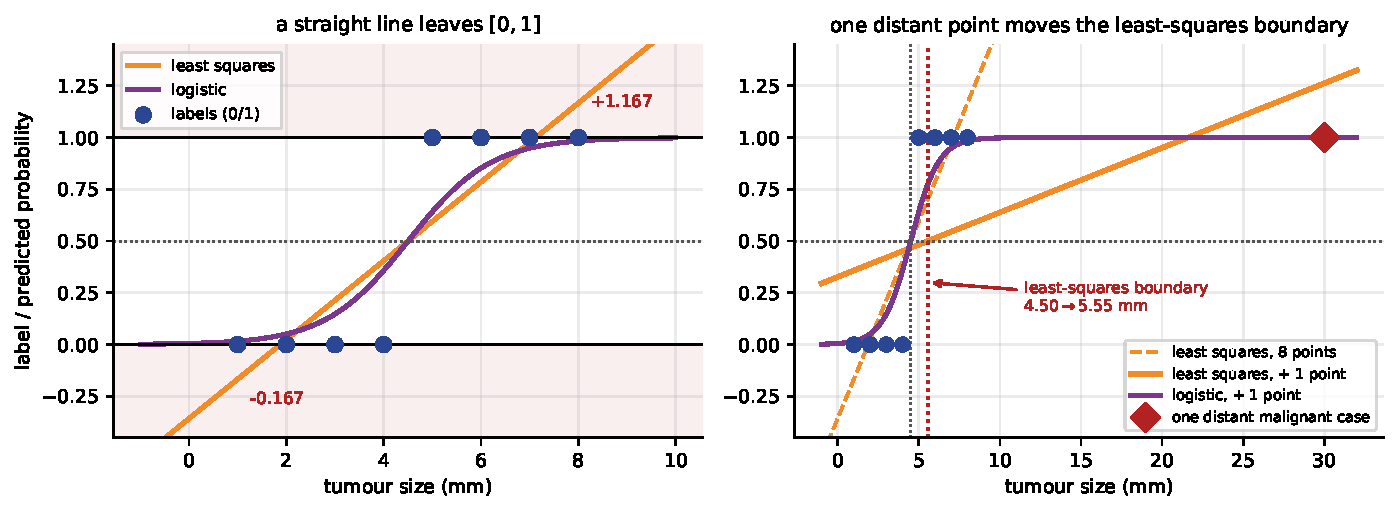
\includegraphics[width=0.88\textwidth]{linfail.pdf}
  \end{center}
  \begin{center}\small
    Left: the shaded bands are the forbidden region, and the orange line
    enters both. Right: the dashed line is least squares on eight points,
    the solid orange line is the same fit with one distant case added.
    \textbf{The purple curve is unmoved.}
  \end{center}
\end{frame}

% =====================================================================
\section[Odds]{Odds, log-odds and the sigmoid}
\label{sec:logit}

\begin{frame}[shrink=8]{Fix the range first, and everything else follows}
  \begin{columns}[T]
    \begin{column}{0.50\textwidth}
      \begin{center}\small
      \begin{tabular}{@{}lll@{}}
        \toprule
        \textbf{Quantity} & \textbf{Range} & \textbf{A line?}\\
        \midrule
        probability $p$ & $(0,1)$ & no\\
        odds $p/(1-p)$ & $(0,\infty)$ & no\\
        log-odds $\ln\frac{p}{1-p}$ & $(-\infty,\infty)$ & \textbf{yes}\\
        \bottomrule
      \end{tabular}
      \end{center}
      \begin{block}{The two moves}
        \begin{enumerate}\small
          \item $p \mapsto p/(1-p)$ stretches $(0,1)$ onto $(0,\infty)$:
            the upper bound is gone.
          \item $\ln(\cdot)$ stretches $(0,\infty)$ onto
            $(-\infty,\infty)$: now \emph{both} bounds are gone.
        \end{enumerate}
      \end{block}
    \end{column}
    \begin{column}{0.46\textwidth}
      \begin{exampleblock}{The whole idea, in one line}
        \centering\large
        $\displaystyle \ln\frac{p}{1-p} = w^{\!\top}x + b$
      \end{exampleblock}
      \begin{block}{The composition has a name}
        \small $\operatorname{logit}(p) = \ln\dfrac{p}{1-p}$, the
        \textbf{link function}: it links the bounded thing we want to the
        unbounded thing a linear model can make. Odds are the bookmaker's
        version of a probability --- $p=0.8$ is odds of $4$.
      \end{block}
      \begin{alertblock}{}
        \small We keep the linear model and change \textbf{what it is a
        model of}. All that remains is (a) inverting that equation and
        (b) finding $w$.
      \end{alertblock}
    \end{column}
  \end{columns}
\end{frame}

\begin{frame}[fragile,shrink=8]{By hand: the odds table you should be able to write out}
\begin{outblk}
 p        odds = p/(1-p)      log-odds = ln(odds)
 0.01          0.0101             -4.5951
 0.10          0.1111             -2.1972
 0.20          0.2500             -1.3863
 0.25          0.3333             -1.0986
 0.50          1.0000             +0.0000
 0.75          3.0000             +1.0986
 0.80          4.0000             +1.3863
 0.90          9.0000             +2.1972
 0.99         99.0000             +4.5951
\end{outblk}
\onslide<2->
\begin{center}\small
  Read it twice. \textbf{$p = 0.5$ is log-odds $0$} --- that is where the
  decision boundary will be. And the table is \textbf{antisymmetric}:
  $\operatorname{logit}(0.2) = -\operatorname{logit}(0.8)$,
  $\operatorname{logit}(0.1) = -\operatorname{logit}(0.9)$. Swapping the two
  classes flips the sign of everything.
\end{center}
\end{frame}

\begin{frame}[shrink=8]{Invert it, and the sigmoid appears}
  Start from the model and solve for $p$. Write $z = w^{\!\top}x + b$.
  \[
    \ln\frac{p}{1-p} = z
    \;\Longrightarrow\;
    \frac{p}{1-p} = e^{z}
    \;\Longrightarrow\;
    p = e^{z} - p\,e^{z}
    \;\Longrightarrow\;
    p\left(1 + e^{z}\right) = e^{z}
  \]
  \[
    \boxed{\;p = \sigma(z) = \frac{e^{z}}{1+e^{z}}
             = \frac{1}{1+e^{-z}}\;}
  \]
  \begin{block}{Three facts to keep}
    \small
    $\sigma(0) = \tfrac12$; \quad
    $\sigma(-z) = 1-\sigma(z)$; \quad
    $\sigma'(z) = \sigma(z)\bigl(1-\sigma(z)\bigr)$.
    \textbf{The sigmoid was not invented. It is what the logit link becomes
    when you turn it round.}
  \end{block}
\end{frame}

\begin{frame}[fragile,shrink=8]{Drawn, and checked in code}
\begin{center}
  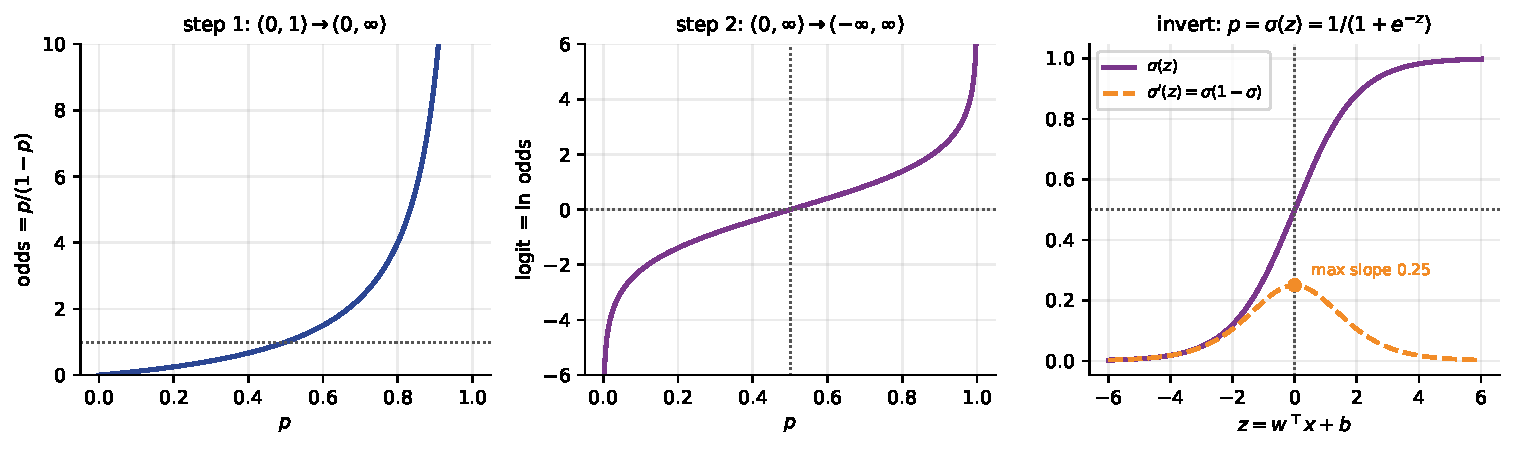
\includegraphics[width=0.86\textwidth]{logitsig.pdf}
\end{center}
\begin{outblk}
logit(sigma(z)) == z ?  True    max error 1.11e-15
sigma(-z) == 1 - sigma(z) ?  True
numerical derivative       0.01766 0.10499 0.19661 0.25000 0.19661 ...
sigma(z) * (1 - sigma(z))  0.01766 0.10499 0.19661 0.25000 0.19661 ...
max difference 6.28e-11
\end{outblk}
\onslide<2->
\begin{center}\small
  The derivative identity is checked against a finite difference, not
  asserted. \textbf{It peaks at $0.25$ where $z=0$}, and that single number
  reappears twice today: in the gradient, and in the ``divide by four'' rule.
\end{center}
\end{frame}

% =====================================================================
\section[Likelihood]{The likelihood, the log-likelihood and the gradient}
\label{sec:mle}

\begin{frame}[shrink=6]{What are we maximising?}
  Each row is a single coin flip whose bias the model supplies:
  \[
    y_i \mid x_i \;\sim\; \text{Bernoulli}\bigl(p_i\bigr), \qquad
    p_i = \sigma(w^{\!\top}x_i + b) .
  \]
  \begin{block}{The Bernoulli trick}
    \[
      P(y_i \mid x_i) = p_i^{\,y_i}\,(1-p_i)^{\,1-y_i}
    \]
    \small One formula for both cases. Put $y_i = 1$: the second factor is
    $(1-p_i)^0 = 1$, leaving $p_i$. Put $y_i = 0$: the first factor is
    $p_i^0 = 1$, leaving $1-p_i$. \textbf{The exponents are switches.}
  \end{block}
  Assuming the rows are independent given $X$, the likelihood is the product:
  \[
    L(w,b) \;=\; \prod_{i=1}^{n} p_i^{\,y_i}\,(1-p_i)^{\,1-y_i} .
  \]
\end{frame}

\begin{frame}[shrink=8]{Take logs --- and meet the cross-entropy loss again}
  A product of $n$ numbers below $1$ underflows; a sum does not. And
  $\ln$ is increasing, so the maximiser is unchanged.
  \[
    \ell(w,b) \;=\; \ln L \;=\;
    \sum_{i=1}^{n}\Bigl[\, y_i \ln p_i + (1-y_i)\ln(1-p_i)\Bigr]
  \]
  \begin{alertblock}{You have already met this function}
    \small Negate it and divide by $n$ and you have the \textbf{binary
    cross-entropy} of L2, which \texttt{sklearn} calls
    \texttt{log\_loss}. Maximising the likelihood \emph{is} minimising the
    cross-entropy. They are the same object seen from two directions ---
    statistics and information theory.
  \end{alertblock}
  \begin{center}\small
    So: $\mathcal{L}(w,b) = -\ell(w,b)$ is the loss we minimise, and the
    optimum is the maximum-likelihood estimate.
  \end{center}
\end{frame}

\begin{frame}[shrink=10]{The gradient, one factor at a time}
  Differentiate $\ell$ with respect to a single weight $w_j$. Chain rule
  through $p_i = \sigma(z_i)$ and $z_i = w^{\!\top}x_i + b$.
  \[
    \frac{\partial \ell}{\partial w_j}
    = \sum_i \underbrace{\left[\frac{y_i}{p_i}
      - \frac{1-y_i}{1-p_i}\right]}_{\partial \ell / \partial p_i}
      \cdot \underbrace{p_i(1-p_i)}_{\partial p_i/\partial z_i}
      \cdot \underbrace{x_{ij}}_{\partial z_i/\partial w_j}
  \]
  Multiply the first two brackets out --- this is the step worth doing on
  paper:
  \[
    \left[\frac{y_i}{p_i} - \frac{1-y_i}{1-p_i}\right] p_i(1-p_i)
    = y_i(1-p_i) - (1-y_i)p_i
    = y_i - y_ip_i - p_i + y_ip_i
    = y_i - p_i .
  \]
  \begin{center}
    \textbf{The $p_i(1-p_i)$ cancels exactly.} That cancellation is the
    reason logistic regression is workable at all.
  \end{center}
\end{frame}

\begin{frame}[shrink=6]{The result: prediction minus truth}
  \begin{exampleblock}{}
    \centering\large
    $\displaystyle
      \frac{\partial \ell}{\partial w_j} = \sum_i (y_i - p_i)\,x_{ij},
      \qquad
      \nabla_w \mathcal{L} = X^{\!\top}(p - y)$
  \end{exampleblock}
  \vspace{0.3em}
  \begin{columns}[T]
    \begin{column}{0.48\textwidth}
      \begin{block}{How to read it}
        \small The gradient is the design matrix transposed, times
        \textbf{the error vector}. Column $j$ of the gradient is
        ``how much feature $j$ correlates with the mistakes I am currently
        making''. The intercept column of ones gives
        $\sum_i (p_i - y_i)$.
      \end{block}
    \end{column}
    \begin{column}{0.48\textwidth}
      \begin{alertblock}{Where you have seen this before}
        \small Least squares has gradient $X^{\!\top}(Xw - y)$ ---
        \emph{also} $X^{\!\top}(\text{prediction} - \text{truth})$. Same
        shape, different prediction. That is not a coincidence: both are
        generalised linear models with their canonical link.
      \end{alertblock}
    \end{column}
  \end{columns}
\end{frame}

\begin{frame}[shrink=8]{By hand: three points, one gradient step}
  $X$ carries an intercept column. Start at $w = (b, w_1) = (0,0)$, so
  every $z_i = 0$ and every $p_i = \sigma(0) = 0.5$.
  \[
    X = \begin{pmatrix} 1 & -2\\ 1 & 0\\ 1 & 2\end{pmatrix},\quad
    y = \begin{pmatrix} 0\\0\\1\end{pmatrix},\quad
    p = \begin{pmatrix} 0.5\\0.5\\0.5\end{pmatrix},\quad
    p - y = \begin{pmatrix} +0.5\\ +0.5\\ -0.5\end{pmatrix}.
  \]
  \[
    X^{\!\top}(p-y) =
    \begin{pmatrix}
      0.5 + 0.5 - 0.5\\[2pt]
      (-2)(0.5) + (0)(0.5) + (2)(-0.5)
    \end{pmatrix}
    = \begin{pmatrix} +0.5\\ -2.0\end{pmatrix}.
  \]
  With $\eta = 0.5$: \quad
  $w \leftarrow (0,0) - 0.5\,(0.5,\,-2.0) = \mathbf{(-0.25,\ +1.0)}$.
  \begin{block}{Then check that it helped}
    \small New $z = (-2.25,\, -0.25,\, 1.75)$, new
    $p = (0.0953,\, 0.4378,\, 0.8520)$, and the log-likelihood moves
    $-2.0794 \to -0.8364$. \textbf{All three probabilities moved towards
    their labels.}
  \end{block}
\end{frame}

\begin{frame}[shrink=8]{Drawn: the same step}
  \begin{center}
    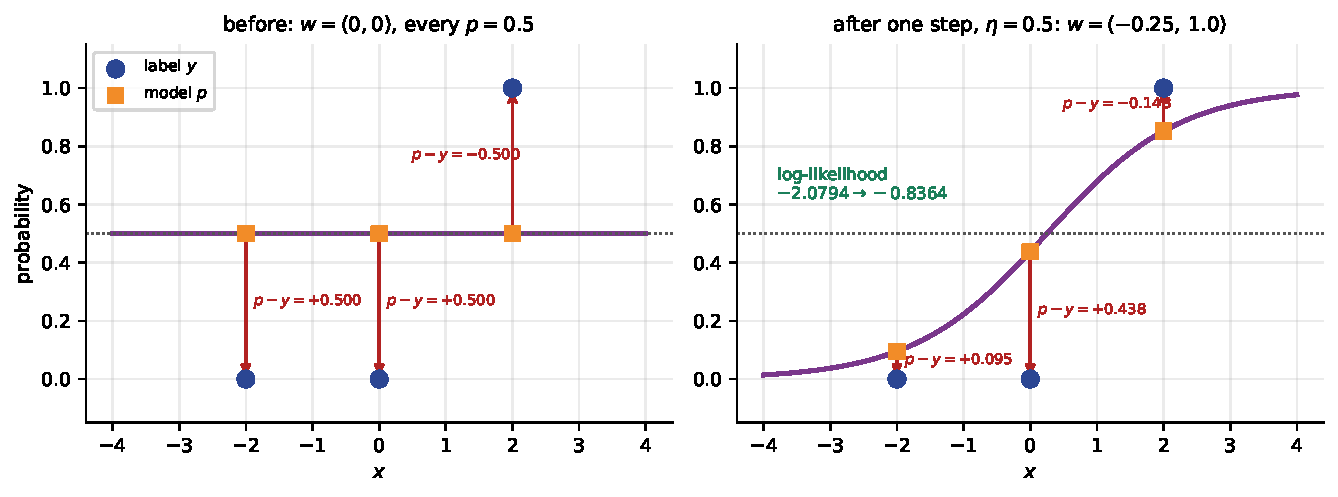
\includegraphics[width=0.86\textwidth]{handstep.pdf}
  \end{center}
  \begin{center}\small
    Blue circles are the labels, orange squares the model, and the red arrow
    on each point is $p - y$: exactly the number that enters the gradient.
    \textbf{Left, every arrow has length $0.5$; right, they are all shorter.}
  \end{center}
\end{frame}

\begin{frame}[fragile,shrink=6]{The same step in code, digit for digit}
\begin{lstlisting}
X = np.array([[1., -2.], [1., 0.], [1., 2.]])   # column 0 = intercept
y = np.array([0., 0., 1.])
w = np.zeros(2)
p = 1 / (1 + np.exp(-(X @ w)))
grad = X.T @ (p - y)
w = w - 0.5 * grad
\end{lstlisting}
\begin{outblk}
p - y            = [ 0.5  0.5 -0.5]
grad = X'(p - y) = [ 0.5 -2. ]
one step, eta = 0.5 :  w <- w - eta * grad = [-0.25  1.  ]
new p = [0.095349 0.437823 0.851953]
log-likelihood  -2.079442 -> -0.836370   (improved by +1.243071)
numerical gradient of the NLL at w = 0: [ 0.5 -2. ]
analytic  X'(p - y)                   : [ 0.5 -2. ]
\end{outblk}
\onslide<2->
\begin{center}\small
  The last two lines are the point of the slide: a \textbf{finite-difference}
  gradient of the loss agrees with the formula we derived. \textbf{If you
  ever doubt a gradient you have derived, check it this way in three lines.}
\end{center}
\end{frame}

\begin{frame}[fragile,shrink=8]{Predict first \#2}
Least squares had a formula. Set the gradient to zero and solve:
$X^{\!\top}Xw = X^{\!\top}y$, one linear system, done.

For logistic regression the same move gives
$X^{\!\top}\bigl(\sigma(Xw) - y\bigr) = 0$.

\begin{center}
  \textbf{Can you solve that for $w$?}
\end{center}
\vspace{0.2em}
\onslide<2->
\begin{outblk}
least squares: beta = (X'X)^-1 X'y = [-1.5  2.2]  -- solved, exactly, in one line
residual gradient X'(Xb - y) = [-0.  0.]

logistic: the same move gives  X'(sigma(Xw) - y) = 0,
          and sigma() cannot be undone to isolate w.
   there is no formula to invert; the equations are transcendental.
   so we iterate.
\end{outblk}
\onslide<3->
\begin{alertblock}{No. And that is a statement about algebra, not about effort}
  \footnotesize $w$ sits \emph{inside} an exponential inside a fraction
  inside a sum. There is no rearrangement that isolates it --- the same
  reason $x e^{x} = 1$ has no elementary solution. \textbf{So we do not
  solve; we descend.} Which is why Unit III came before Unit V.
\end{alertblock}
\end{frame}

\begin{frame}[fragile,shrink=8]{But we can promise you will not get stuck}
The Hessian of the log-likelihood is
$H = -X^{\!\top}SX$ with $S = \operatorname{diag}\bigl(p_i(1-p_i)\bigr)$,
and every $p_i(1-p_i) > 0$.
\begin{outblk}
w = [0. 0.]        eigenvalues of H  [-7.  -1.5]         all < 0 : True
w = [-0.5  1. ]    eigenvalues of H  [-2.2368 -0.6133]   all < 0 : True
w = [ 2. -3.]      eigenvalues of H  [-0.4823 -0.0235]   all < 0 : True
\end{outblk}
\onslide<2->
\begin{alertblock}{Negative definite everywhere $\Rightarrow$ strictly concave}
  \footnotesize For any $v \ne 0$,
  $v^{\!\top}Hv = -\sum_i p_i(1-p_i)(x_i^{\!\top}v)^2 < 0$ whenever $X$ has
  full column rank. \textbf{One maximum, no local traps, no random
  restarts.} Compare a neural network, where none of that is true --- this
  is the whole reason logistic regression is still the default first model.
\end{alertblock}
\onslide<3->
\begin{center}\small
  Concavity guarantees the optimum is \emph{unique}. It does not guarantee
  the optimum is \emph{finite} --- hold that thought for the last section.
\end{center}
\end{frame}

\begin{frame}[shrink=8]{Drawn: one hill, and two ways up it}
  \begin{center}
    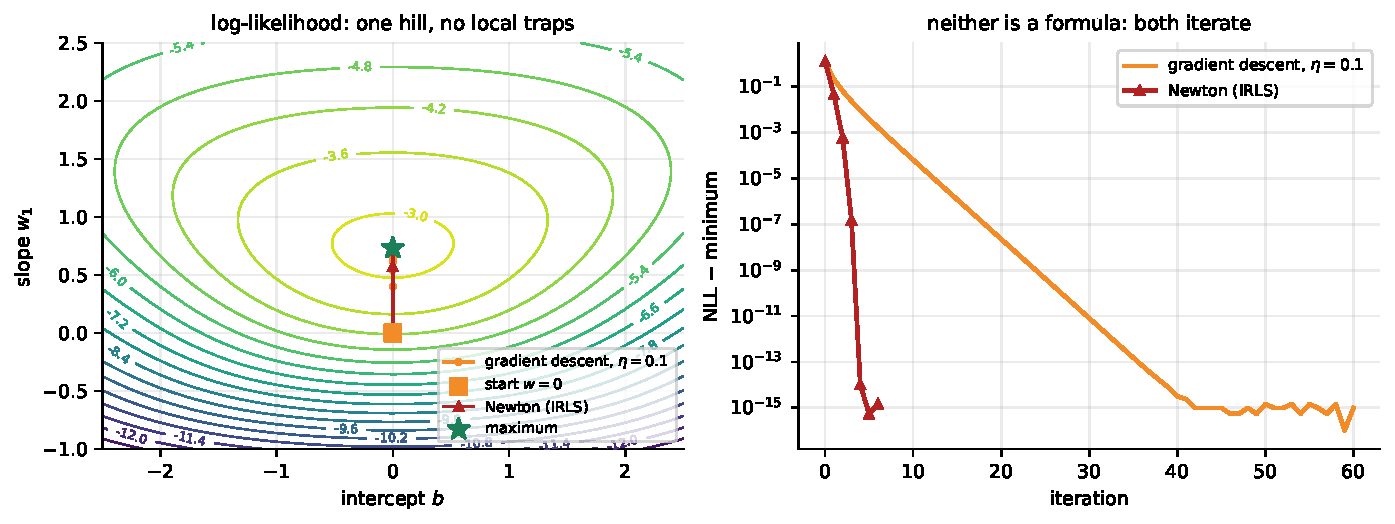
\includegraphics[width=0.86\textwidth]{likelihood.pdf}
  \end{center}
  \begin{center}\small
    Six points, two parameters. Left: the contours of $\ell$ close on a
    single peak. Orange is gradient descent at $\eta = 0.1$; red is Newton's
    method, which uses $H$ and arrives in about five steps. Right: the same
    two runs on a log scale. \textbf{Neither is a formula.}
  \end{center}
\end{frame}

\begin{frame}[fragile,shrink=8]{Run it to the end, and compare with the library}
\begin{outblk}
  iter        b          w1        NLL      |grad|max
     1  +0.000000  +0.400000   3.094797    1.43e+00
     2  -0.000000  +0.543158   2.941879    7.28e-01
    10  +0.000000  +0.726183   2.876549    2.08e-02
   100  -0.000000  +0.732488   2.876484    2.22e-16
sklearn LogisticRegression(penalty=None):  b -0.000000  w1 +0.732488
our gradient descent after 20000 steps  :  b -0.000000  w1 +0.732488
agreement to 11 decimal places
\end{outblk}
\onslide<2->
\begin{outblk}
Newton step 1:  b +0.000000  w1 +0.571429  |grad| 4.000e+00
Newton step 3:  b -0.000000  w1 +0.732187  |grad| 6.322e-02
Newton step 5:  b -0.000000  w1 +0.732488  |grad| 2.516e-07
Newton step 6:  b -0.000000  w1 +0.732488  |grad| 1.588e-14
\end{outblk}
\onslide<3->
\begin{center}\small
  \textbf{Eleven decimal places} between fourteen lines of \texttt{numpy} and
  \texttt{scikit-learn}. Newton's method --- which statisticians call
  \textbf{IRLS} --- needs six steps rather than a hundred, because it uses
  the curvature we just computed.
\end{center}
\end{frame}

% =====================================================================
\section[Coefficients]{Reading the coefficients}
\label{sec:odds}

\begin{frame}[shrink=6]{What a coefficient means}
  Increase $x_j$ by one unit. Then $z$ increases by $\beta_j$, so
  \[
    \frac{\text{new odds}}{\text{old odds}}
    = \frac{e^{\,z+\beta_j}}{e^{\,z}} = e^{\beta_j}.
  \]
  \begin{exampleblock}{}
    \centering\large
    $e^{\beta_j}$ is a \textbf{multiplicative} change in the \textbf{odds}.
  \end{exampleblock}
  \vspace{0.2em}
  \begin{alertblock}{It is not a change in probability, and it is not additive}
    \small ``$\beta = 0.7$, so the chance goes up by $70\%$'' is wrong twice
    over. The correct sentence is: \textbf{one more unit of $x_j$ multiplies
    the odds by $e^{0.7} = 2.01$, whatever those odds were.} The change in
    \emph{probability} depends entirely on where you started.
  \end{alertblock}
  \begin{center}\small
    $\beta_j > 0 \Rightarrow e^{\beta_j} > 1$ (odds up);\;
    $\beta_j = 0 \Rightarrow e^{\beta_j} = 1$ (no effect);\;
    $\beta_j < 0 \Rightarrow e^{\beta_j} < 1$ (odds down).
  \end{center}
\end{frame}

\begin{frame}[fragile,shrink=8]{By hand: one coefficient, five starting points}
Take $\beta = \ln 2 = 0.693147$, so the odds ratio is exactly $2$.
\begin{outblk}
 start p    start odds   new odds    new p      change in p
   0.05        0.0526     0.1053    0.0952      +0.0452
   0.20        0.2500     0.5000    0.3333      +0.1333
   0.50        1.0000     2.0000    0.6667      +0.1667
   0.80        4.0000     8.0000    0.8889      +0.0889
   0.95       19.0000    38.0000    0.9744      +0.0244
\end{outblk}
\onslide<2->
\begin{center}\small
  Do the middle row on paper: odds $1 \to 2$, so
  $p = 2/(1+2) = 0.6667$. \textbf{The odds ratio is $2.0$ in every row. The
  change in probability ranges from $+0.024$ to $+0.167$} --- a factor of
  $6.8$ --- from one and the same coefficient.
\end{center}
\onslide<3->
\begin{center}\small
  This is why a paper reports odds ratios and a patient wants probabilities.
  \textbf{They are different questions and you must not mix the answers.}
\end{center}
\end{frame}

\begin{frame}[shrink=8]{Drawn: the same arrow, five places on the curve}
  \begin{center}
    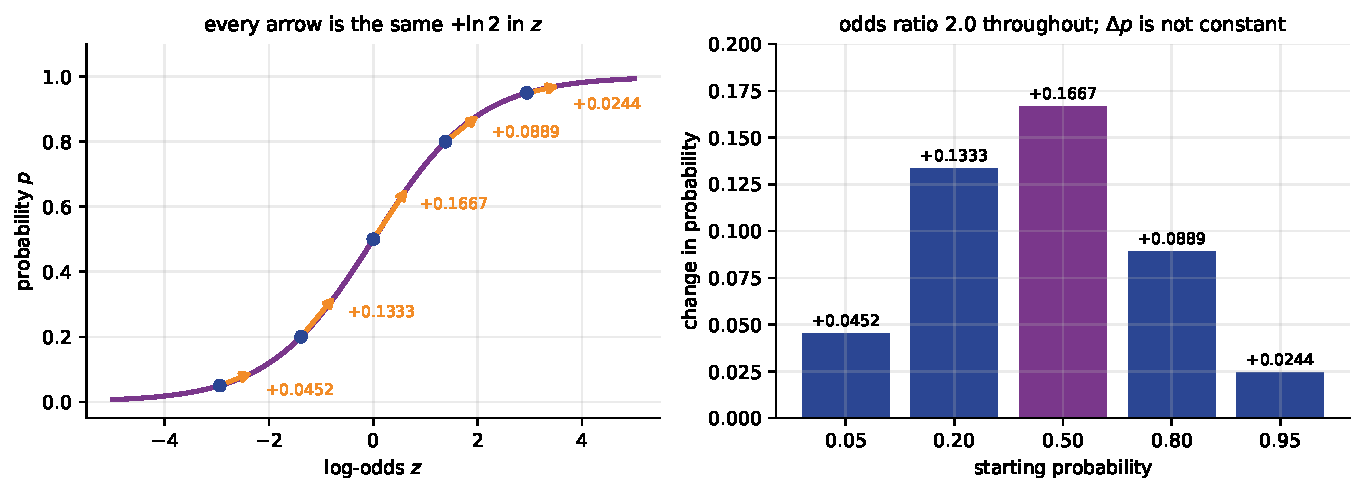
\includegraphics[width=0.86\textwidth]{oddsratio.pdf}
  \end{center}
  \begin{center}\small
    Every orange arrow is the same horizontal shift of $\ln 2 = 0.693$ in
    $z$. The vertical distance it buys depends on how steep the sigmoid is
    where you are standing --- \textbf{steepest at $p = 0.5$, nearly flat at
    the ends.}
  \end{center}
\end{frame}

\begin{frame}[fragile,shrink=8]{Predict first \#3}
\texttt{load\_breast\_cancer}, $569$ patients. Fit malignancy on
\texttt{mean radius} alone, in millimetres. The fitted model is
\[
  \ln\frac{p}{1-p} = -15.2521 + 1.0340\,r .
\]
\begin{center}
  \textbf{One extra millimetre of radius. By how much does the probability
  of malignancy rise?}
\end{center}
\vspace{0.2em}
\onslide<2->
\begin{outblk}
exp(b1) = 2.8124   -- the ODDS multiply by 2.81 per mm, always
   radius 10.0 -> 11.0 mm : p 0.0073 -> 0.0203  (+0.0130), odds x 2.8124
   radius 14.0 -> 15.0 mm : p 0.3152 -> 0.5642  (+0.2490), odds x 2.8124
   radius 17.5 -> 18.5 mm : p 0.9450 -> 0.9797  (+0.0347), odds x 2.8124
   radius 20.0 -> 21.0 mm : p 0.9956 -> 0.9984  (+0.0028), odds x 2.8124
\end{outblk}
\onslide<3->
\begin{alertblock}{The question has no single answer, and that is the answer}
  \footnotesize From $+0.28$ percentage points to $+24.9$ --- a factor of
  \textbf{eighty-nine} --- depending on the patient. The odds ratio,
  $2.8124$, is the same in every row. \textbf{Divide-by-four rule:} the
  steepest slope is $\beta/4 = 0.2585$, i.e.\ about
  $\mathbf{26}$ percentage points per mm, and never more.
\end{alertblock}
\end{frame}

\begin{frame}[shrink=8]{Drawn: a real fit, and thirty odds ratios}
  \begin{center}
    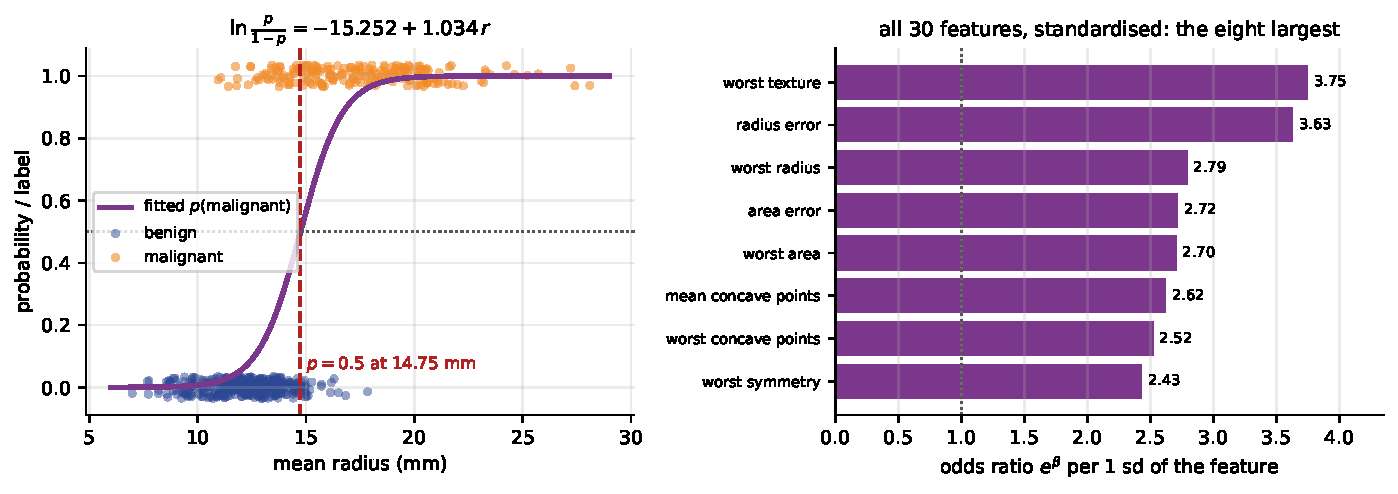
\includegraphics[width=0.88\textwidth]{bcradius.pdf}
  \end{center}
  \begin{center}\small
    Left: one feature in its own units --- the $50\%$ point falls at
    $14.75$ mm, and this single-feature model is already $87.87\%$ accurate.
    Right: all thirty features standardised, so each bar reads
    \textbf{``odds multiplier per one standard deviation''}.
    \textbf{Standardise before you compare coefficients, or you are
    comparing units.}
  \end{center}
\end{frame}

% =====================================================================
\section[Threshold]{The decision threshold is a choice}
\label{sec:thresh}

\begin{frame}[fragile,shrink=8]{$0.5$ is a default, not a law}
\texttt{predict()} rounds at $0.5$. Nothing in the derivation says it must.
Held-out set: $171$ patients, $64$ of them malignant.
\begin{outblk}
thresh   TN   FP   FN   TP   accuracy  precision  recall     F1
 0.10    93   14    1   63    0.9123     0.8182   0.9844  0.8936
 0.25    95   12    3   61    0.9123     0.8356   0.9531  0.8905
 0.40   101    6    3   61    0.9474     0.9104   0.9531  0.9313
 0.50   103    4    4   60    0.9532     0.9375   0.9375  0.9375
 0.60   106    1    5   59    0.9649     0.9833   0.9219  0.9516
 0.75   107    0    6   58    0.9649     1.0000   0.9062  0.9508
 0.90   107    0    8   56    0.9532     1.0000   0.8750  0.9333
ROC AUC 0.9917 -- unchanged by the threshold, because it averages over all
\end{outblk}
\onslide<2->
\begin{alertblock}{The model never changed. Only the rounding rule did}
  \footnotesize Same $171$ probabilities on every row. At $0.10$ we miss
  \textbf{one} cancer and raise $14$ false alarms; at $0.90$ we miss
  \textbf{eight} and raise none. \textbf{The best accuracy on this split is
  $0.9708$ at a threshold of $0.62$, not at $0.50$.} Which row is right is a
  clinical question, not a statistical one.
\end{alertblock}
\end{frame}

\begin{frame}[shrink=8]{Drawn: the trade-off you are actually choosing}
  \begin{center}
    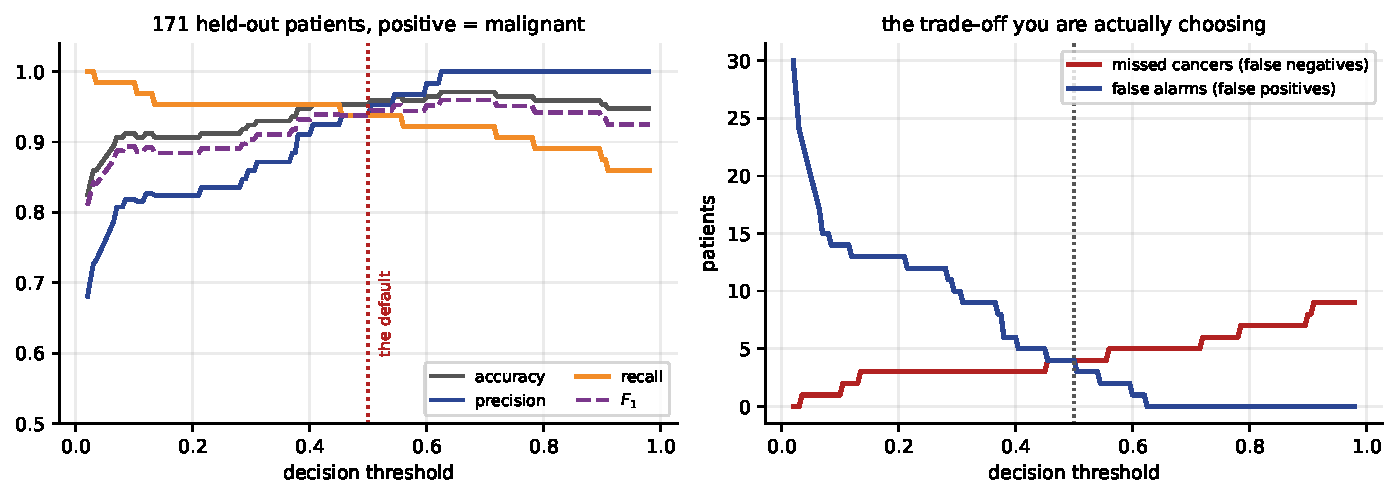
\includegraphics[width=0.88\textwidth]{threshold.pdf}
  \end{center}
  \begin{center}\small
    Left: four metrics as the threshold sweeps. Precision and recall move in
    opposite directions by construction. Right: the same picture in
    patients rather than ratios. \textbf{Choose the threshold from the cost
    of the two mistakes, then report which one you chose.}
  \end{center}
\end{frame}

% =====================================================================
\section[Multiclass]{More than two classes}
\label{sec:multi}

\begin{frame}[shrink=6]{From sigmoid to softmax}
  With $K$ classes, give each class its own linear score
  $z_k = w_k^{\!\top}x + b_k$ and normalise:
  \[
    P(y = k \mid x) \;=\; \frac{e^{z_k}}{\sum_{m=1}^{K} e^{z_m}}
    \qquad\text{(softmax)}
  \]
  \begin{columns}[T]
    \begin{column}{0.48\textwidth}
      \begin{block}{Two properties, free of charge}
        \small Every term is positive, and they sum to $1$ by
        construction. So the output is a genuine distribution over the $K$
        classes, not $K$ unrelated scores.
      \end{block}
      \begin{block}{And $K = 2$ gives back the sigmoid}
        \small Put $z_0 = 0$ (only differences matter). Then
        $P(y=1) = e^{z_1}/(1+e^{z_1}) = \sigma(z_1)$.
      \end{block}
    \end{column}
    \begin{column}{0.48\textwidth}
      \begin{exampleblock}{The loss is the same loss}
        \small
        $\displaystyle \mathcal{L} = -\sum_i \sum_k
          \mathbb{1}[y_i = k]\,\ln P(y_i = k \mid x_i)$ ---
        \textbf{categorical cross-entropy}, the multi-class version of L2's
        loss, and the gradient is again $X^{\!\top}(P - Y)$ with $Y$
        one-hot.
      \end{exampleblock}
      \begin{alertblock}{The alternative: one-vs-rest}
        \small Fit $K$ separate binary models, ``class $k$ against
        everything else'', then normalise. Simpler, but the $K$ fits never
        talk to each other.
      \end{alertblock}
    \end{column}
  \end{columns}
\end{frame}

\begin{frame}[fragile,shrink=8]{Softmax against one-vs-rest, measured}
\begin{lstlisting}
soft = make_pipeline(StandardScaler(), LogisticRegression(max_iter=10000))
ovr  = make_pipeline(StandardScaler(),
                     OneVsRestClassifier(LogisticRegression(max_iter=10000)))
\end{lstlisting}
\begin{outblk}
softmax (multinomial): coef_ shape (3, 4), intercept_ shape (3,)
first three flowers, softmax probabilities:
   [0.984703 0.015297 0.      ]  sum 1.000000
   [0.943549 0.056451 0.      ]  sum 1.000000
5-fold accuracy  softmax 0.9600    one-vs-rest 0.9267
cross-entropy (log_loss) softmax 0.129534   one-vs-rest 0.280427
with K = 2 the softmax collapses to the sigmoid: True
\end{outblk}
\onslide<2->
\begin{center}\small
  \textbf{One row of coefficients per class}, and the probabilities sum to
  one exactly. On iris, softmax beats one-vs-rest by $0.033$ of accuracy and
  by more than a factor of two on cross-entropy --- because it was trained
  to produce a \emph{joint} distribution rather than three separate ones.
\end{center}
\end{frame}

\begin{frame}[shrink=8]{Drawn: three classes, one normalisation}
  \begin{center}
    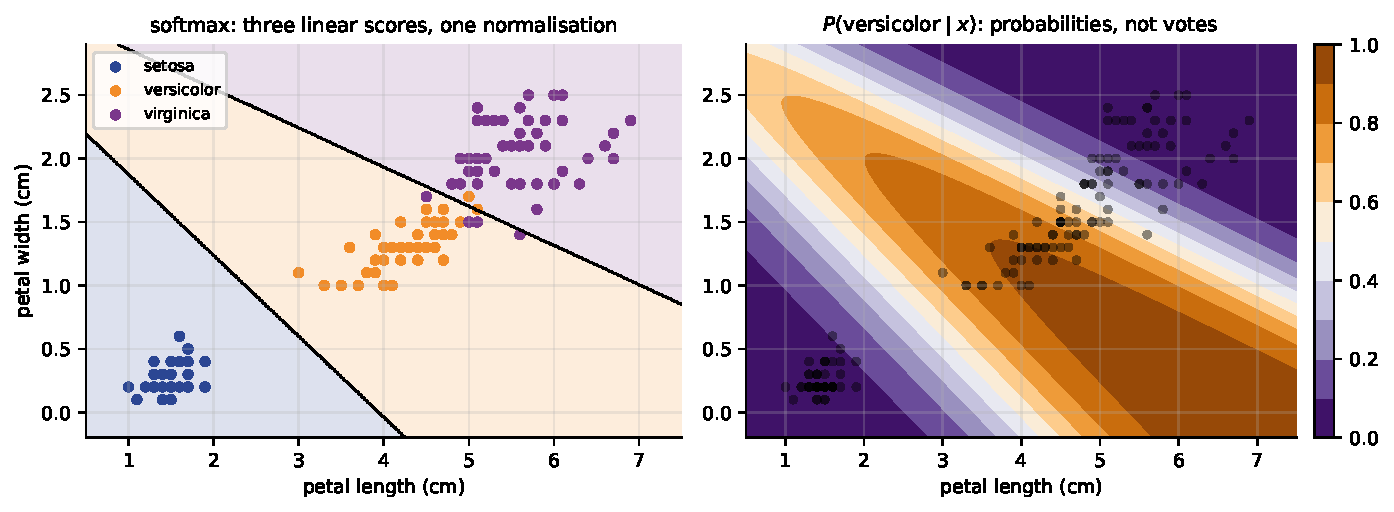
\includegraphics[width=0.88\textwidth]{softmax.pdf}
  \end{center}
  \begin{center}\small
    Left: the boundaries are straight lines, because each pair of classes is
    separated where $z_j = z_k$, which is linear in $x$. Right: the
    probability surface for one class. \textbf{Logistic regression is a
    linear classifier that reports its uncertainty.}
  \end{center}
\end{frame}

% =====================================================================
\section[Separation]{Perfect separation}
\label{sec:sep}

\begin{frame}[fragile,shrink=8]{Predict first \#4}
Six points on a line. Every $x < 0$ is class $0$; every $x > 0$ is class
$1$. \textbf{A perfect split exists.} Run unpenalised gradient descent on
the negative log-likelihood and keep going.

\begin{center}
  \textbf{What does $w_1$ settle down to?}
\end{center}
\vspace{0.2em}
\onslide<2->
\begin{outblk}
  steps        w1          NLL        p at x = +1
     10      3.3921   6.851e-02   0.967457475172
    100      4.8035   1.647e-02   0.991865702976
   1000      6.9326   1.952e-03   0.999025489499
  10000      9.2132   1.994e-04   0.999900294931
 100000     11.5132   1.999e-05   0.999990003302
 200000     12.2062   9.998e-06   0.999995000852
\end{outblk}
\onslide<3->
\begin{alertblock}{It does not settle. There is no maximum}
  \footnotesize Every ten-fold increase in steps adds about $2.3 = \ln 10$
  to $w_1$: the likelihood approaches $1$ only as
  $\lVert w\rVert \to \infty$. The optimum is at infinity, so the MLE
  \textbf{does not exist}. This is \emph{perfect separation}, and it is the
  one case where concavity does not save you.
\end{alertblock}
\end{frame}

\begin{frame}[fragile,shrink=8]{What the library does, and what fixes it}
\begin{outblk}
max_iter   |w1|        NLL          warning
       3     1.8045  3.670e-01    ConvergenceWarning
       5     2.9086  1.125e-01    ConvergenceWarning
      10     6.2700  3.788e-03    ConvergenceWarning
      25    16.6643  1.158e-07    ConvergenceWarning
     100    31.2204  5.607e-14    (none)
the warning text: lbfgs failed to converge after 5 iteration(s) (status=1):
\end{outblk}
\onslide<2->
\begin{outblk}
       C      |w1|       b        NLL      p at x = +1
    0.01    0.0561  -0.0000   3.83339    0.514017
    1.00    1.1044  -0.0000   0.85240    0.751084
  100.00    3.9462  +0.0000   0.03905    0.981038
accuracy is 1.0000 at every C -- separation is not a fitting failure
\end{outblk}
\onslide<3->
\begin{alertblock}{The fix is regularisation, which is the next-but-one lecture}
  \footnotesize The L2 penalty adds $\tfrac{1}{2C}\lVert w\rVert^2$, so an
  infinite $w$ costs infinitely much and \textbf{the optimum becomes finite
  again}. Note that \texttt{scikit-learn} penalises \emph{by default} ---
  which is why you may never have met this bug. \textbf{Ridge and lasso:
  L12.}
\end{alertblock}
\end{frame}

\begin{frame}[fragile,shrink=8]{And it happens on real data}
\texttt{load\_iris}, setosa against versicolor, petal length alone.
\begin{outblk}
   largest setosa 1.9 cm, smallest versicolor 3.0 cm -- separable: True
   unpenalised   coefficient     +51.8263  intercept    -127.9249
   default L2    coefficient      +2.8999  intercept      -7.8853
   the unpenalised coefficient is 18 times larger
   both score accuracy 1.0000 and 1.0000 -- the fit is not the problem
   unpenalised p at petal length 2.5 cm: 0.8376399347
   penalised    p at petal length 2.5 cm: 0.3462536277
\end{outblk}
\onslide<2->
\begin{alertblock}{$0.84$ against $0.35$ for the same flower}
  \footnotesize Both models classify all $100$ flowers correctly, so no
  accuracy figure would ever tell you something was wrong. But a coefficient
  of $\mathbf{51.8}$ per centimetre is not a finding, and in the gap between
  $1.9$ and $3.0$ cm --- where you have \textbf{no data} --- the two models
  disagree completely. \textbf{Read your coefficients, not just your score.}
\end{alertblock}
\end{frame}

\begin{frame}[shrink=8]{Drawn: the runaway, and the brake}
  \begin{center}
    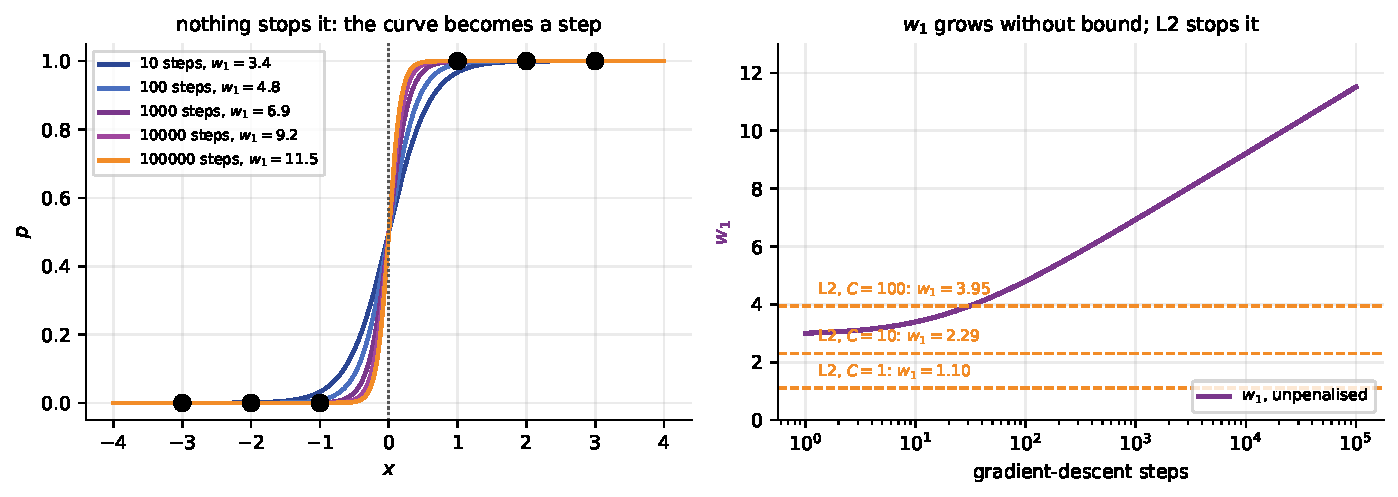
\includegraphics[width=0.88\textwidth]{separation.pdf}
  \end{center}
  \begin{center}\small
    Left: the fitted curve at five points along the same run --- it is
    turning into a step function. Right: $w_1$ against the number of steps,
    on a log axis, next to where each L2 penalty stops it.
    \textbf{Nothing in the unpenalised problem draws a line.}
  \end{center}
\end{frame}

% =====================================================================
\section{Summary}
\label{sec:summary}

\begin{frame}[shrink=16]{Summary --- ten lines}
  \begin{enumerate}\small
    \item Least squares on $0/1$ labels gave $\hat y = -0.1667$ and
      $+1.1667$ on eight points, and \textbf{one distant, correct malignant
      case moved its boundary from $4.50$ to $5.55$ mm} and cost it a
      patient. Logistic regression did not move at all.
    \item A probability lives in $(0,1)$, odds in $(0,\infty)$, log-odds in
      $(-\infty,\infty)$. \textbf{Model the log-odds}:
      $\ln\frac{p}{1-p} = w^{\!\top}x + b$.
    \item Invert that and the sigmoid falls out:
      $p = 1/(1+e^{-z})$, with $\sigma(0)=\tfrac12$,
      $\sigma(-z)=1-\sigma(z)$ and $\sigma' = \sigma(1-\sigma)$, maximum
      $0.25$.
    \item Bernoulli likelihood
      $\prod p_i^{y_i}(1-p_i)^{1-y_i}$; log-likelihood
      $\sum [y_i\ln p_i + (1-y_i)\ln(1-p_i)]$, which is
      \textbf{minus the cross-entropy of L2}.
    \item $\dfrac{\partial\ell}{\partial w_j} = \sum_i (y_i - p_i)x_{ij}$,
      so $\nabla\mathcal{L} = X^{\!\top}(p-y)$: \textbf{prediction minus
      truth}. The $p(1-p)$ from the chain rule cancels exactly.
    \item Three points, $w=0$, gave $X^{\!\top}(p-y) = (0.5, -2.0)$ and
      $w \leftarrow (-0.25, 1.0)$; the log-likelihood moved
      $-2.0794 \to -0.8364$. The code agrees to eleven decimals with
      \texttt{sklearn}.
    \item \textbf{No closed form}: $\sigma$ cannot be inverted out of
      $X^{\!\top}(\sigma(Xw)-y)=0$. But $H = -X^{\!\top}SX$ is negative
      definite, so $\ell$ is \textbf{strictly concave} --- one maximum, no
      restarts. Newton (IRLS) took $6$ steps to gradient descent's $100$.
    \item $e^{\beta}$ multiplies the \textbf{odds}, not the probability.
      $\beta = \ln 2$ moved $p$ by $+0.0244$ from $0.95$ and $+0.1667$ from
      $0.50$. On breast\_cancer, $e^{\beta} = 2.8124$ per mm of radius, and
      one extra mm was worth between $+0.28$ and $+24.9$ percentage points.
    \item The threshold is \textbf{yours}. At $0.10$: one missed cancer, $14$
      false alarms. At $0.90$: eight missed, none. Best accuracy was
      $0.9708$ at $0.62$, not at $0.50$. AUC $0.9917$ throughout.
    \item Softmax generalises the sigmoid to $K$ classes and beat one-vs-rest
      $0.9600$ to $0.9267$ on iris. And when the classes are
      \textbf{perfectly separable the MLE does not exist}: $w_1$ grew past
      $12$ and kept going, $51.8$ on real iris data. \textbf{Regularisation
      is the fix, and that is L12.}
  \end{enumerate}
\end{frame}

\begin{frame}[shrink=3]{Before the next lecture}
  \begin{columns}[T]
    \begin{column}{0.48\textwidth}
      \begin{block}{Read}
        \texttt{notes.pdf} --- the derivation written out in full, every
        step, because it is examinable; plus \textbf{10 practice questions
        with worked solutions}.
      \end{block}
      \begin{block}{Do}
        Questions 2, 4 and 5. Question 4 is one gradient step by hand on two
        points; question 5 is an odds-ratio sentence that most people get
        wrong the first time.
      \end{block}
    \end{column}
    \begin{column}{0.48\textwidth}
      \begin{exampleblock}{Next: multiple linear regression}
        Many predictors at once, partial and standardised coefficients, and
        model validation. \textbf{The gradient
        $X^{\!\top}(\hat y - y)$ you met today reappears there with
        $\hat y = Xw$.}
      \end{exampleblock}
      \begin{alertblock}{And a habit to start now}
        Whenever you report a logistic coefficient, report $e^{\beta}$ next
        to it and say the sentence out loud: \emph{``one more unit
        multiplies the odds by \dots''} If the sentence sounds wrong, the
        number is being misread.
      \end{alertblock}
    \end{column}
  \end{columns}
  \begin{center}
    \small Materials: \texttt{\AMLRepoURL}
  \end{center}
  \slidesources{\AMLUnitVSources}
\end{frame}

\end{document}
